\documentclass[10pt]{beamer}

\usetheme{metropolis}
\usepackage{appendixnumberbeamer}

\usepackage{booktabs}
\usepackage[scale=2]{ccicons}
\usepackage{graphicx}
\usepackage{hyperref}
\usepackage{circuitikz}
\usepackage{pdflscape}
\usepackage{smartdiagram}

\usepackage{color}
\usepackage{listings}

\lstset{
	basicstyle=\footnotesize\ttfamily,
    keepspaces=true,
    showstringspaces=false,
    language=PHP,
    commentstyle=\ttfamily,
}

\usepackage[OT4]{polski}
\usepackage[utf8]{inputenc}

\usepackage{pgfplots}
\usepgfplotslibrary{dateplot}

\usepackage{xspace}
\newcommand{\themename}{\textbf{\textsc{metropolis}}\xspace}

\setbeamertemplate{frame footer}{}
\setbeamertemplate{frame numbering}{}

\usetikzlibrary{shapes,arrows}

\tikzstyle{decision} = [diamond, draw, fill=blue!20, 
    text width=4.5em, text badly centered, node distance=3cm, inner sep=0pt]
\tikzstyle{block} = [rectangle, draw, fill=blue!20, 
    text width=5em, text centered, rounded corners, minimum height=4em]
\tikzstyle{line} = [draw, -latex']
\tikzstyle{cloud} = [draw, ellipse,fill=red!20, node distance=3cm,
    minimum height=2em]


\title{Analiza ruchu w aplikacji webowej}

\subtitle{Projektowanie i programowanie systemów internetowych I}
\author{mgr inż. Krzysztof Rewak}
\date{\today}
\institute{Wydział Nauk Technicznych i Ekonomicznych \\ Państwowa Wyższa Szkoła Zawodowa im. Witelona w Legnicy}

\begin{document}

\maketitle

\begin{frame}{Plan prezentacji}
  \setbeamertemplate{section in toc}[sections numbered]
  \tableofcontents[hideallsubsections]
\end{frame}


\begin{frame}{Dawne czasy}
	\begin{figure}[t]
		\centering
		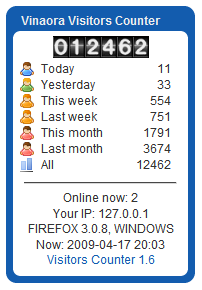
\includegraphics[width=.5\linewidth]{counter.png}
	\end{figure}
\end{frame}

\begin{frame}{Dawne czasy}
	Czasy, w których takie liczniki gości można było znaleźć bardzo często, słusznie już minęły.
	
	Ludzie wykształcili od tego czasu wiele przydatnych narzędzi. Przynajmniej część z nich warto znać.
\end{frame}

\begin{frame}{Jak to ugryźć?}
	Gdzie można podpiąć nasłuchiwanie ruchu w naszej aplikacji?
	
	Praktycznie rzecz biorąc wszędzie: zarówno na webowym backendzie, webowym frontendzie czy aplikacji mobilnej.
\end{frame}

\begin{frame}{Co ugryźć?}
	Czego można dowiedzieć się podczas nasłuchiwania ruchu w naszej aplikacji?
	
	Wszystkiego. W granicach rozsądku. Zazwyczaj.
\end{frame}

\section{Klasyczna analityka}

\begin{frame}[fragile]{Badanie zapytań HTTP}
	Większość frameworków oferuje proste sposoby na wydobycie informacji o IP klienta.
	
	Przykładowo:

\begin{lstlisting}
public function returnIP(Request $request): JsonResponse {
    return respone()->json(["ip" => $request->ip());
}
\end{lstlisting}
\end{frame}

\begin{frame}{IP}
	A znając IP można zbadać już naprawdę wiele ciekawych rzeczy.
\end{frame}

\begin{frame}{IP}
	\begin{figure}[t]
		\centering
		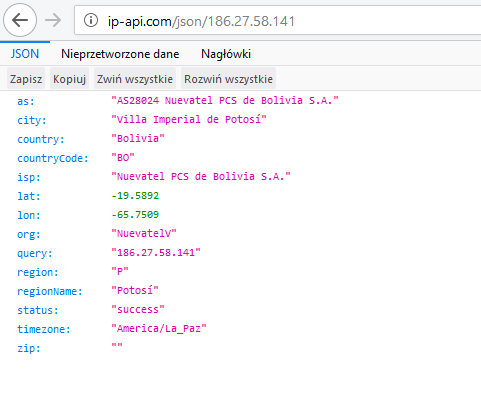
\includegraphics[width=.75\linewidth]{ip.png}
	\end{figure}
\end{frame}

\begin{frame}{Logowanie zdarzeń}
	Warto rozważyć logowanie ruchu na stronie wewnątrz własnej aplikacji. Jest to proste do wykonania, ale warto pamiętać o kilku szczegółach.
\end{frame}

\begin{frame}{Logowanie zdarzeń}
	\begin{figure}[t]
		\centering
		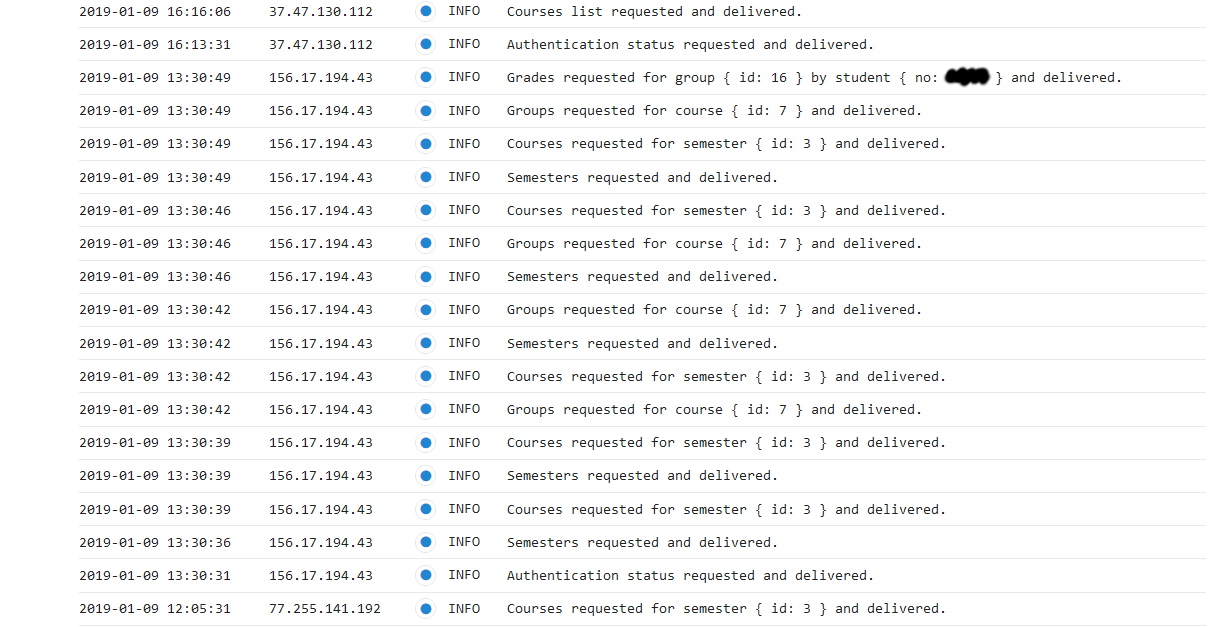
\includegraphics[width=\linewidth]{logs.png}
	\end{figure}
\end{frame}

\begin{frame}{Logowanie zdarzeń}
	\begin{itemize}
	\item serwery HTTP (Apache, nginx) najczęściej robią to już za nas w postaci access- i errorlogów;
	\item warto zastanowić się czy lepiej logować dane do pliku czy do bazy danych;
	\item jeszcze bardziej warto się zastanowić po jakim czasie dane należy usuwać;
	\end{itemize}
\end{frame}

\begin{frame}{RFC 5424}
	Istnieje nawet standard RFC 5424, który opisuje poziomy logów:
	\begin{itemize}
	\item 100 DEBUG
	\item 200 INFO
	\item 250 NOTICE
	\item 300 WARNING
	\item 400 ERROR
	\item 500 CRITICAL
	\item 550 ALERT
	\item 600 EMERGENCY
	\end{itemize}
\end{frame}

\begin{frame}{Logowanie zdarzeń}
	Co można zrobić z takimi logami? 
	\begin{itemize}
	\item zbadać zerwane linki;
	\item sprawdzić czy ktoś nie próbował się włamać do zastrzeżonych miejsc;
	\item sprawdzić popularność produktów;
	\item zbadać w którym miejscu procesu zakupowego klient najczęściej rezygnuje;
	\item i setki innych zastosowań...
	\end{itemize}
\end{frame}

\section{Przydatna analityka}

\begin{frame}{Google Analytics}
	Królem webowej analityki od lat jest \textbf{Google Analytics}.
\end{frame}

\begin{frame}{Google Analytics}
	Stosowane na frontendzie, Google Analytics jest bardzo proste w użyciu.
	
	W bazowej wersji wymaga jedynie załączenia odpowiedniego skryptu, a następnie wywoływania jednej metody \texttt{ga()}.
\end{frame}

\begin{frame}[fragile]{Google Analytics (ałć!)}
\begin{lstlisting}
<script>
(function(i,s,o,g,r,a,m){
i['GoogleAnalyticsObject']=r;i[r]=i[r]||function(){
(i[r].q=i[r].q||[]).push(arguments)
},i[r].l=1*new Date();a=s.createElement(o),
m=s.getElementsByTagName(o)[0];a.async=1;
a.src=g;m.parentNode.insertBefore(a,m)
})(window,document,'script',
'https://www.google-analytics.com/analytics.js','ga');

ga('create', 'UA-4815162342-1', 'auto');
ga('send', 'pageview');
</script>
\end{lstlisting}
\end{frame}

\begin{frame}[fragile]{Google Analytics}
	Oczywiście każdy sensowniejszy javascriptowy framework już od dawna ma własne wrappery, które niestraszą zminifikowanym kodem.
	
	Przykładowa implementacja GA w Vue.js:

\begin{lstlisting}
Vue.use(VueAnalytics, {
	id: "UA-4815162342-1",
	checkDuplicatedScript: true,
	router
})
\end{lstlisting}
\end{frame}

\begin{frame}{Google Analytics}
	\begin{figure}[t]
		\centering
		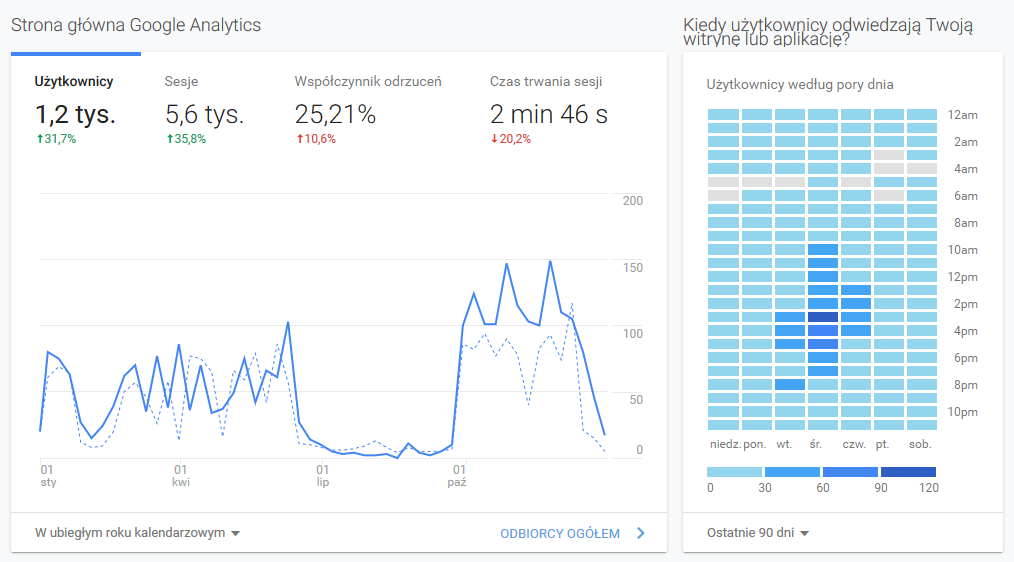
\includegraphics[width=\linewidth]{ga1.png}
	\end{figure}
\end{frame}

\begin{frame}{Google Analytics}
	\begin{figure}[t]
		\centering
		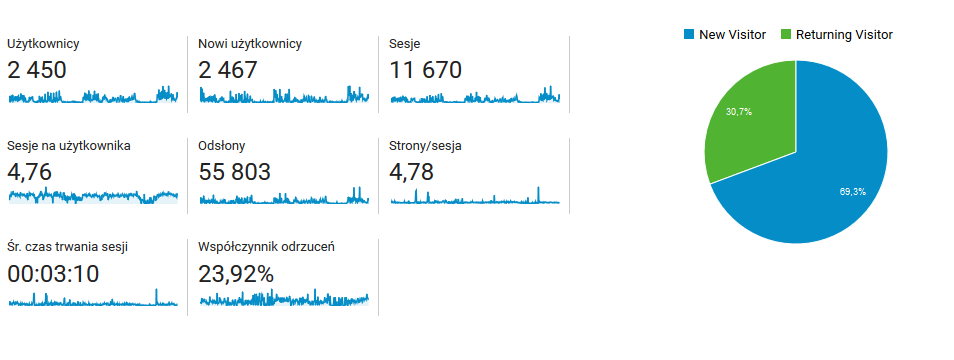
\includegraphics[width=\linewidth]{ga2.png}
	\end{figure}
\end{frame}

\begin{frame}{Google Analytics}
	\begin{figure}[t]
		\centering
		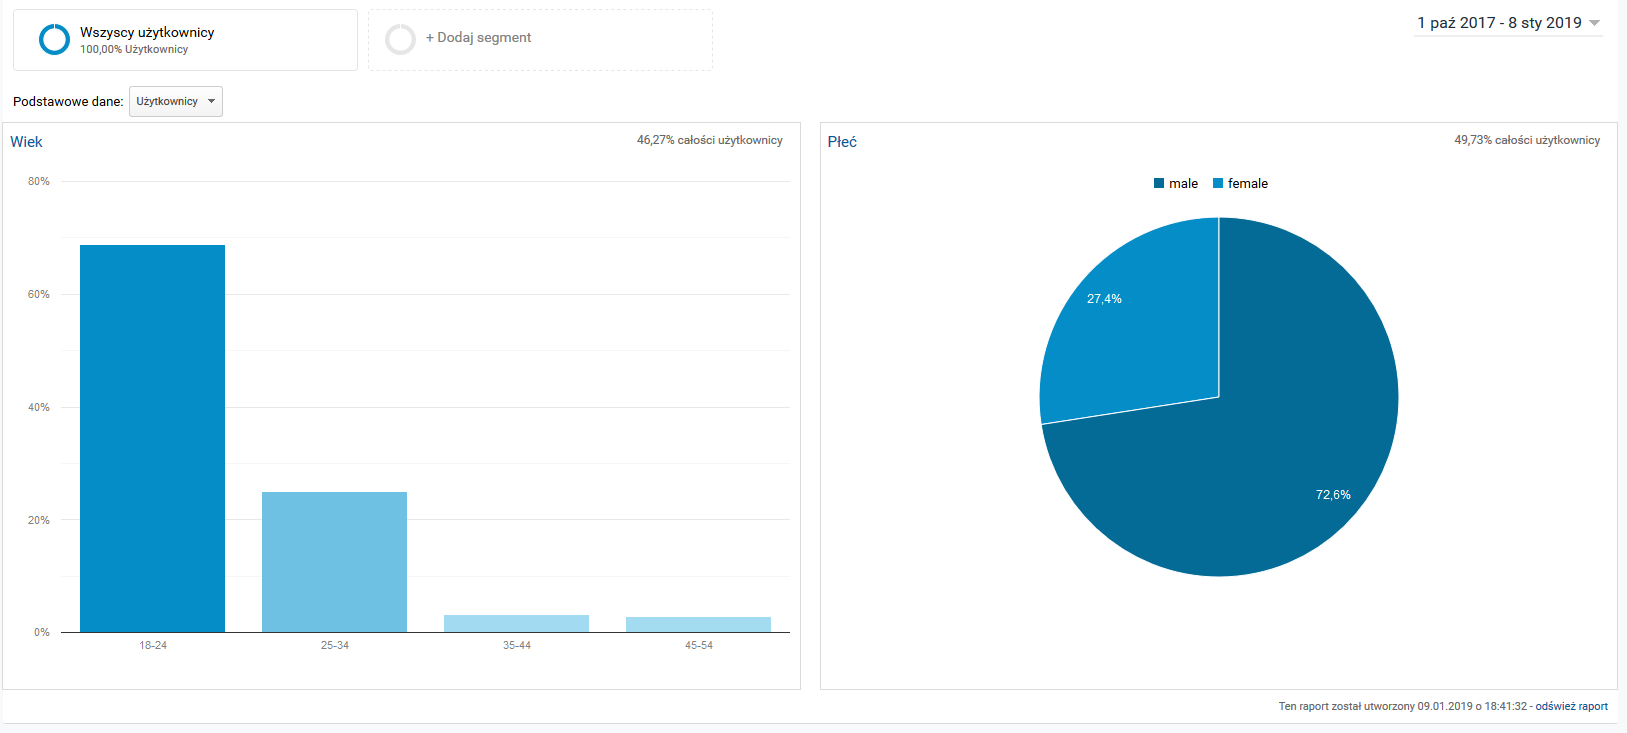
\includegraphics[width=\linewidth]{ga3.png}
	\end{figure}
\end{frame}

\begin{frame}{Google Analytics}
	\begin{figure}[t]
		\centering
		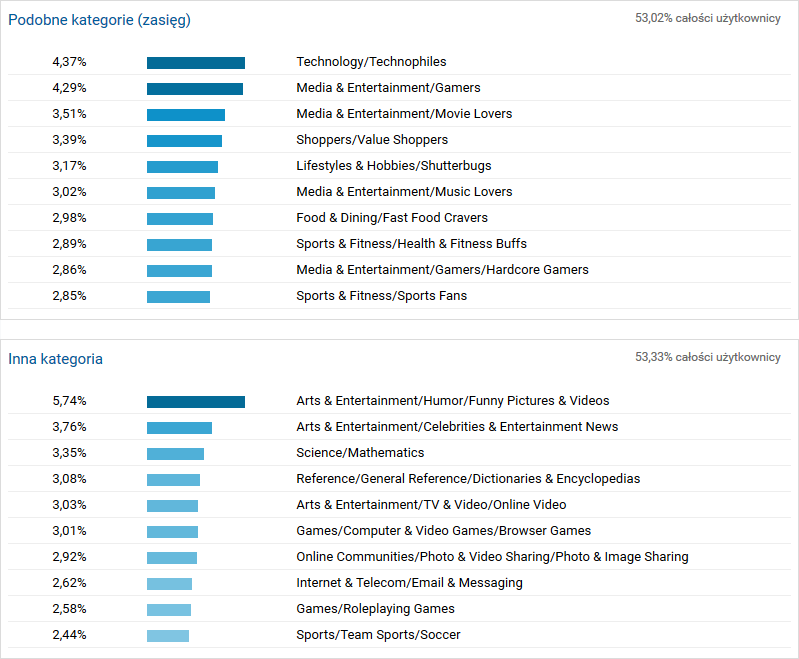
\includegraphics[width=.8\linewidth]{ga4.png}
	\end{figure}
\end{frame}

\begin{frame}{Google Analytics}
	\begin{figure}[t]
		\centering
		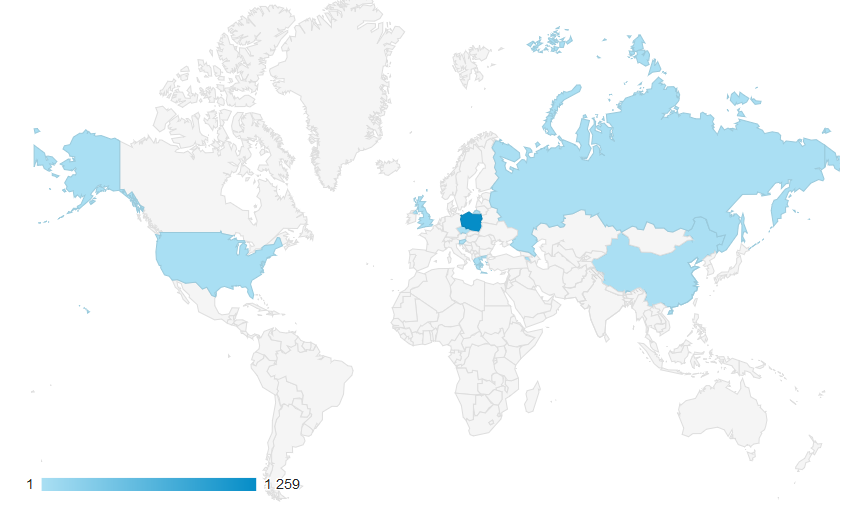
\includegraphics[width=\linewidth]{ga5.png}
	\end{figure}
\end{frame}

\begin{frame}{Google Analytics}
	\begin{figure}[t]
		\centering
		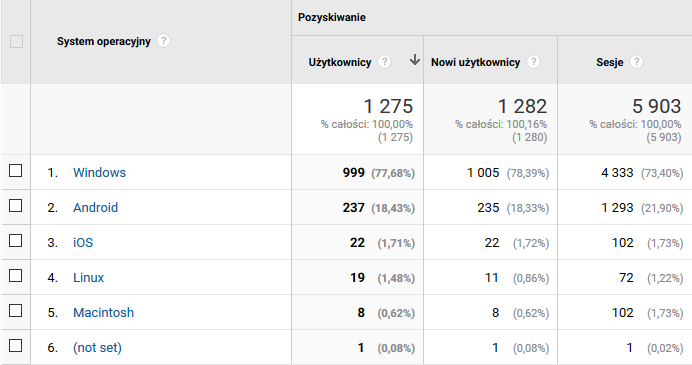
\includegraphics[width=\linewidth]{ga6.png}
	\end{figure}
\end{frame}

\begin{frame}{Google Analytics}
	\begin{figure}[t]
		\centering
		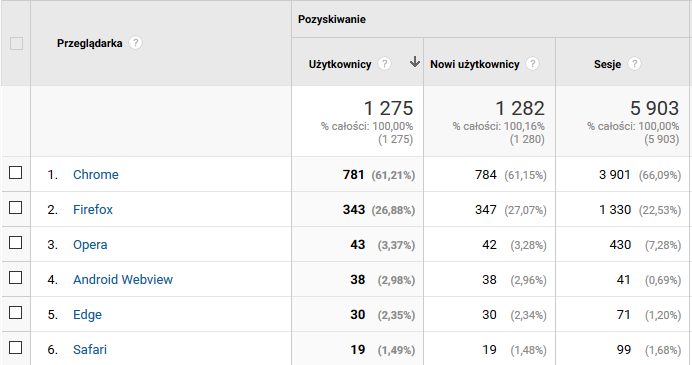
\includegraphics[width=\linewidth]{ga7.png}
	\end{figure}
\end{frame}

\begin{frame}{Google Analytics}
	\begin{figure}[t]
		\centering
		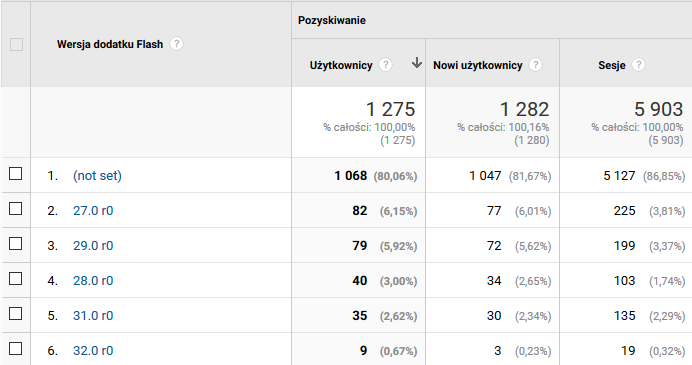
\includegraphics[width=\linewidth]{ga8.png}
	\end{figure}
\end{frame}

\begin{frame}{Google Analytics}
	\begin{figure}[t]
		\centering
		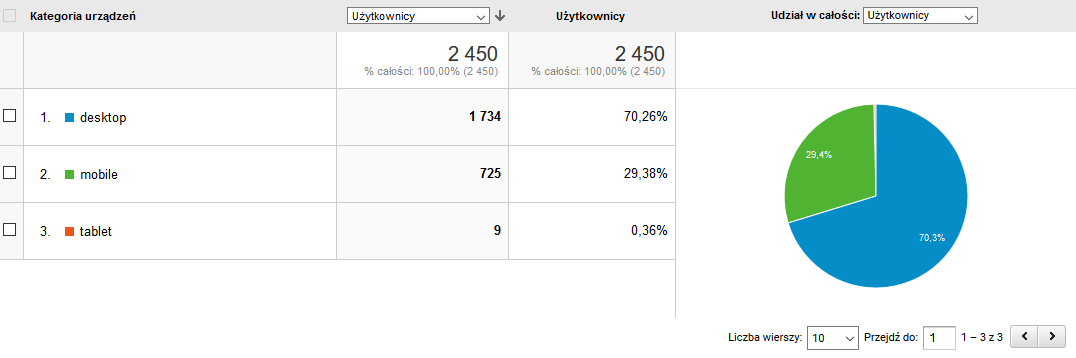
\includegraphics[width=\linewidth]{ga9.png}
	\end{figure}
\end{frame}

\begin{frame}{Google Analytics}
	\begin{figure}[t]
		\centering
		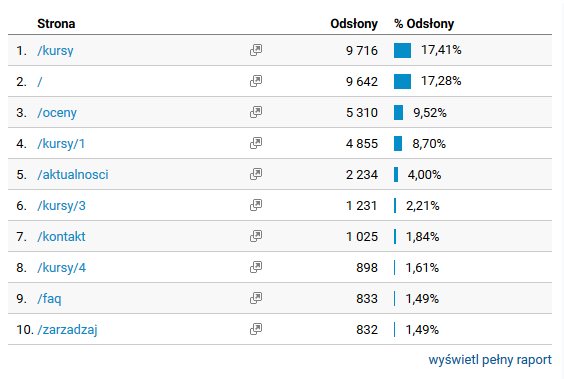
\includegraphics[width=.8\linewidth]{ga10.png}
	\end{figure}
\end{frame}

\begin{frame}{Google Analytics}
	\begin{figure}[t]
		\centering
		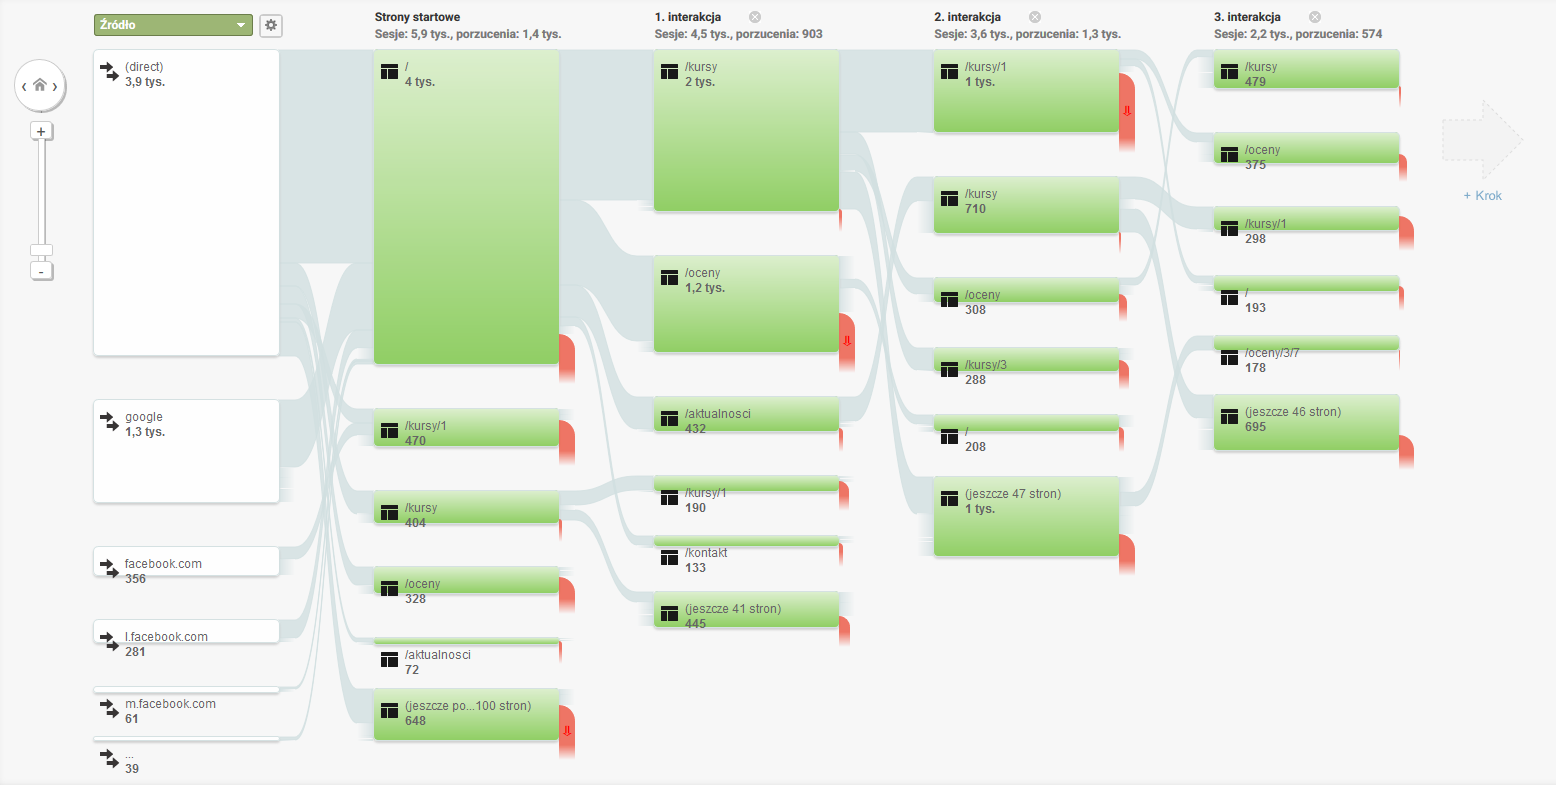
\includegraphics[width=\linewidth]{ga11.png}
	\end{figure}
\end{frame}

\section{Straszna analityka}

\begin{frame}{Inne rozwiązania}
	Istnieje cała masa innych rozwiązań. 
	
	Popularnym może być New Relic (raczej wykorzystywany po stronie backendu), Kissmetrics (do śledzenia konkretnych użytkowników) czy CrazyEgg (do generowania heatmap).
\end{frame}

\begin{frame}{Inne rozwiązania}
	Należy pamiętać, że granica prywatności to rzecz bardzo względna i może się okazać, że aplikacja śledzi naprawdę każdy ruch użytkownika.
\end{frame}

\begin{frame}{Inne rozwiązania}
	Jakim problemem (od strony technicznej) jest sprawdzenie w jakie miejsca na stronie klika się najczęściej?
\end{frame}

\begin{frame}{Inne rozwiązania}
	Jakim problemem (od strony technicznej) jest zrobienie zrzutu ekranu użytkownika?
\end{frame}

\begin{frame}{Inne rozwiązania}
	Jakim problemem (od strony moralnej) jest nagranie całej sesji użytkownika?
\end{frame}

\begin{frame}[standout]
	Czas na eksperyment!
\end{frame}

\section{Podsumowanie}

\begin{frame}{Bibliografia i ciekawe źródła}
  
	\begin{thebibliography}{9}
		
		\bibitem{gof}
		\url{https://tools.ietf.org/html/rfc5424}
	
	\end{thebibliography}

\end{frame}

\appendix

\begin{frame}[standout]
	Pytania?
\end{frame}

\begin{frame}{}

	Kod prezentacji dostępny jest w repozytorium git pod adresem \texttt{https://bitbucket.org/krewak/pwsz-ppsi} \\ \ \\

	\begin{figure}
		\centering
		\href{https://bitbucket.org/krewak/pwsz-ppsi}{
			
\includegraphics[width=.15\textwidth]{../_template/bitbucket.png}
		}
	\end{figure}
	
	Wszystkie informacje dot. kursu dostępne są pod adresem \texttt{http://pwsz.rewak.pl/kursy/4} \\ \ \\

	\begin{figure}
		\centering
		\href{http://pwsz.rewak.pl/kursy/3}{
			
\includegraphics[width=.15\textwidth]{../_template/rewak.png}
		}
	\end{figure}

\end{frame}

\end{document}
